\subsection{Etapa de definición}

Los esquemas openEHR son transformados a la sintaxis de ADL, creándose los arquetipos openEHR de recursos FHIR. Las estructuras de los recursos son representadas usando las clases openEHR CLUSTER para los tipos de datos FHIR complejos y openEHR ELEMENT para los tipos de datos FHIR primitivos.

Continuando con el ejemplo, el arquetipo creado a partir del esquema openEHR del recurso SimplifiedPatient se ilustra en la figura \ref{fig:definition}.

\begin{figure}
  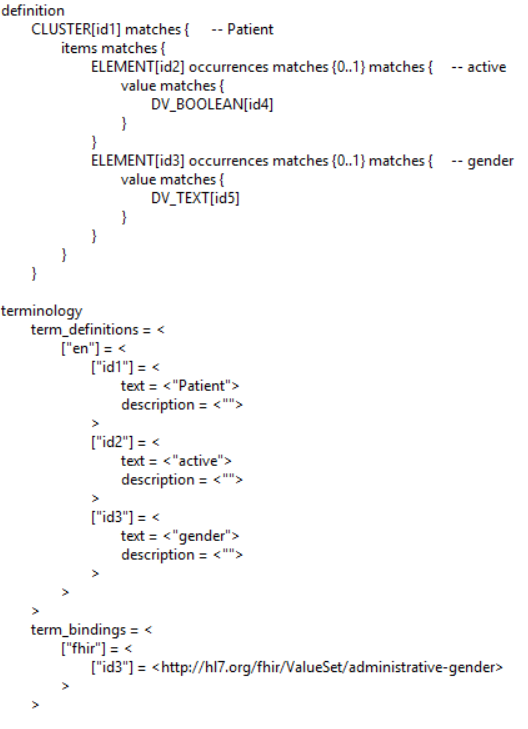
\includegraphics[scale=0.5]{./images/definition}
  \caption{Arquetipo del recurso SimplifiedPatient}
  \label{fig:definition}
\end{figure}

Los nuevos arquetipos creados pueden ser considerados como arquetipos de integración similar al utilizado en la estrategia de integración basada en arquetipos \cite{openEHRIntegration}. En esta estrategia, los arquetipos de integración son utilizados para expresar los datos de las instancias de los recursos FHIR como instancias del modelo de referencia de openEHR. Estos arquetipos pueden ser utilizados por software openEHR o bien mapeados a arquetipos existentes utilizando herramientas de modelados de arquetipos.
